
\iftrue % Make iffalse to create a handout.
\documentclass[xcolor=svgnames]{beamer}
\else
\documentclass[xcolor=svgnames, handout]{beamer}
\fi

\usepackage[utf8]    {inputenc}
\usepackage[T1]      {fontenc}
\usepackage[english] {babel}
\usepackage{tikz}
\usepackage{amsmath,amsfonts,graphicx}
\usepackage{beamerleanprogress}
\usepackage{minted}

\usemintedstyle{borland}
\newmintedfile[cFile]{c}{
bgcolor=lightgray,
fontfamily=tt,
fontsize=\tiny,
frame=leftline,
framerule=0.4pt,
framesep=2mm,
funcnamehighlighting=true,
gobble=0,
linenos=true,
mathescape=false
numberblanklines=true,
numbersep=5pt,
obeytabs=false,
showspaces=false,
showtabs=false,
tabsize=4,
texcl=false,
}

\usemintedstyle{borland}
\newmintedfile[cppFile]{cpp}{
bgcolor=lightgray,
fontfamily=tt,
fontsize=\tiny,
frame=leftline,
framerule=0.4pt,
framesep=2mm,
funcnamehighlighting=true,
gobble=0,
linenos=true,
mathescape=false
numberblanklines=true,
numbersep=5pt,
obeytabs=false,
showspaces=false,
showtabs=false,
tabsize=4,
texcl=false,
}

\title
    [Design Principles\hspace{2em}]
    {Design Principles and Design Patterns}

\author
    [Ryan Bartling]
    {D. Ryan Bartling}

\AtBeginSection[]
{
    \begin{frame}<beamer>{\secname}
        \tableofcontents[currentsection]
    \end{frame}
}

\begin{document}

%%%%%%%%%%%%%%%%%%%%%%%%%%%%%%%%%%%%%%%%%%%%%%%%%%%%%%%%%%%%%%%%%%%%%%%%%%%%%%%%


% Clean build fails. Make the next line \iffalse to build.
% Then, change back to \iftrue to build the full document.
\iftrue
\maketitle

%%%%%%%%%%%%%%%%%%%%%%%%%%%%%%%%%%%%%%%%%%%%%%%%%%%%%%%%%%%%%%%%%%%%%%%%%%%%%%%%

\setcounter{tocdepth}{1}
\begin{frame}{Outline}
    \tableofcontents
\end{frame}

%%%%%%%%%%%%%%%%%%%%%%%%%%%%%%%%%%%%%%%%%%%%%%%%%%%%%%%%%%%%%%%%%%%%%%%%%%%%%%%%

\section{Introduction}

%%%%%%%%%%%%%%%%%%%%%%%%%%%%%%%%%%%%%%%%%%%%%%%%%%%%%%%%%%%%%%%%%%%%%%%%%%%%%%%%

\begin{frame}{Architecture and Dependencies}
    \centering
    \includegraphics[height=0.95\textheight]{dependency}
\end{frame}
% Notes:
% I present here a general architectural pattern that I frequently use.
% The arrows here point in the direction of dependency.  E.g. lib.c depends on
% lib.h.  The application depends on lib.h, but not on lib.c.  A platform
% specific implementation of class_a.c (such as a UART driver) depends on the
% platform.

%%%%%%%%%%%%%%%%%%%%%%%%%%%%%%%%%%%%%%%%%%%%%%%%%%%%%%%%%%%%%%%%%%%%%%%%%%%%%%%%

\section[Rotting Code]{Symptoms of Rotting Design}

%%%%%%%%%%%%%%%%%%%%%%%%%%%%%%%%%%%%%%%%%%%%%%%%%%%%%%%%%%%%%%%%%%%%%%%%%%%%%%%%

\begin{frame}{\secname}
    \begin{enumerate}
        \pause \item Rigidity % Unflexible
        \pause \item Fragility % Easily broken
        \pause \item Immobility % Not reusable
        \pause \item Viscosity % Resistance to flow
    \end{enumerate}
\end{frame}
% Notes:
% A code smell is that feeling that there is something not quite right with the
% code.  That intuition that there is something here that doesn't work.  Smells
% can also apply to the organisation that produces the code.  And many times a
% combination of smells can arise from a single issue.  The smells discused
% below are not all there is, but they are four big ones that can help guide
% conversation during code review.

% Rigidity describes code that resists efforts to change.
% Fragility describes code that easily breaks when worked with.  Often in subtle
% and unexpected ways.

% Immobility describes code that defies efforts to reuse.
% Viscosity  describes code whose design resists the flow of work.  Code whose
% design crumbles under efforts to adapt to changing requirements.

%%%%%%%%%%%%%%%%%%%%%%%%%%%%%%%%%%%%%%%%%%%%%%%%%%%%%%%%%%%%%%%%%%%%%%%%%%%%%%%%

\subsection{Rigidity}
\newcommand{\background}{brick}

%%%%%%%%%%%%%%%%%%%%%%%%%%%%%%%%%%%%%%%%%%%%%%%%%%%%%%%%%%%%%%%%%%%%%%%%%%%%%%%%

{%
\usebackgroundtemplate{%
    \tikz\node[opacity=1.0]{%
        \includegraphics<handout:0>[height=\paperheight,width=\paperwidth]{%
            \background}};}%
\begin{frame}<handout:0>{\subsecname}
\end{frame}
}

{%
\usebackgroundtemplate{%
    \tikz\node[opacity=0.2]{%
        \includegraphics<handout:0>[height=\paperheight,width=\paperwidth]{%
            \background}};}%
\begin{frame}{\subsecname}

    \begin{itemize}
        \item \href{https://www.merriam-webster.com/dictionary/rigid}
            {Deficient in or devoid of flexibility} \pause
        \item Software for which extra effort is expended in order to make
            changes. \pause
        \item The system is hard to change because every change forces many
            other changes to other parts of the system.
    \end{itemize}
\end{frame}
}

% Notes:
% For each smell, I will provide an english definition of the word, a definition
% more specific to software, and a phrase or feeling that fits with the smell.
% I will then try and illustrate the smell with some code examples.

% Rigidity is defined as that which is deficient in or devoid of flexibility.
% I find this definition unsatisfying as it is defined as an opposite of another
% word.

% To give more meaning, we can state it's definition as rigid software is
% software for which extra effort is required and expended in order to make
% changes.  How much extra effort can become a measure of rigidity.

% If you find yourself saying "the system is hard to change because every change
% forces many other changes to other parts of the system," then you may have
% found yourself working on some rigid software.

%%%%%%%%%%%%%%%%%%%%%%%%%%%%%%%%%%%%%%%%%%%%%%%%%%%%%%%%%%%%%%%%%%%%%%%%%%%%%%%%

{%
\usebackgroundtemplate{%
    \tikz\node[opacity=0.2]{%
        \includegraphics<handout:0>[height=\paperheight,width=\paperwidth]{%
            \background}};}%
\begin{frame}{\subsecname}

    How it happens
    \begin{itemize}
        \pause \item Overly procedural code
        \pause \item Lack of abstractions
        \pause \item Solving a generic problem with implementation specific details
        \pause \item Spreading a single responsibility throughout several parts
        \pause \item When components need a lot of knowledge about each other in
            order to function
    \end{itemize}
\end{frame}
}

% Notes:
% What leads to rigidity?

% Give class time to answer.

% Code written in a way that focuses on how the goal is accomplished rather than on breaking it up into smaller goals until each goal is trivially solved.

% This is can be seen by a general lack of abstractions.  Many different levels of a problem space are addressed in a single function or module.

% This can result in a fairly generic problem (e.g. implementing a queue) with many implementation specific details (e.g. UART registers for the transmition queue).

% Even worse, a single responsibility can be spread accross many different modules.  Such as through an over reliance of globals that are read or modified accross several portions of code.

% When many components require intiment knowledge of each other modules, you have a rigid system.

%%%%%%%%%%%%%%%%%%%%%%%%%%%%%%%%%%%%%%%%%%%%%%%%%%%%%%%%%%%%%%%%%%%%%%%%%%%%%%%%

{%
\usebackgroundtemplate{%
    \tikz\node[opacity=0.2]{%
        \includegraphics<handout:0>[height=\paperheight,width=\paperwidth]{%
            \background}};}%
\begin{frame}{\subsecname}
    \begin{minipage}{\columnwidth}
        \cFile{rigid.c}
    \end{minipage}
\end{frame}
}

% Notes:
% This is oversimplified slideware.  Many smells of rigidity are more subtle and often cannot be fit on a single screen.

% In this case, the rigidity is highlighted by the comments of the writer of the code.

% It's also highlighted by the defensive preprocessor checks between lines at the end of the snippet.  Note, without those checks, it would be arguably fragile in addition to being rigid, so these checks, in and of themselves are not bad, and quite helpful.

% The comments and preprocessor checks, if anything highlight that the code is written by an engineer with some experience, even if they aren't at a senior or principle level, yet.

%%%%%%%%%%%%%%%%%%%%%%%%%%%%%%%%%%%%%%%%%%%%%%%%%%%%%%%%%%%%%%%%%%%%%%%%%%%%%%%%

{%
\usebackgroundtemplate{%
    \tikz\node[opacity=0.2]{%
        \includegraphics<handout:0>[height=\paperheight,width=\paperwidth]{%
            \background}};}%
\begin{frame}{\subsecname}
    \begin{minipage}{\columnwidth}
        \cFile{rigid_change.c}
    \end{minipage}
\end{frame}
}

% Notes:
% We can see that making a change to the number of bits used from the ADC triggers changes to three other lines of code.  The first change, doesn't actually get caught by the checks.  It's not until the next line gets changed that the preprocessor checks get triggered and help future developer.

%%%%%%%%%%%%%%%%%%%%%%%%%%%%%%%%%%%%%%%%%%%%%%%%%%%%%%%%%%%%%%%%%%%%%%%%%%%%%%%%

{%
\usebackgroundtemplate{%
    \tikz\node[opacity=0.2]{%
        \includegraphics<handout:0>[height=\paperheight,width=\paperwidth]{%
            \background}};}%
\begin{frame}{\subsecname}
    Refactor to reduce rigidity
    \begin{minipage}{\columnwidth}
        \cFile{rigid_fix.c}
    \end{minipage}
\end{frame}
}

% This can be solved by defining relationships in code rather than in comments and checks (or not at all).

% While this is a somewhat trivial example in order to fit on the slide, it is inspired by real code.  Principles can be applied on both small and large scale in order to reduce rigidity at all levels.

%%%%%%%%%%%%%%%%%%%%%%%%%%%%%%%%%%%%%%%%%%%%%%%%%%%%%%%%%%%%%%%%%%%%%%%%%%%%%%%%

{%
\usebackgroundtemplate{%
    \tikz\node[opacity=0.2]{%
        \includegraphics<handout:0>[height=\paperheight,width=\paperwidth]{%
            \background}};}%
\begin{frame}<handout:0>{\subsecname}
    \centering
    \includegraphics[height=0.1\textheight]{rigid1}
\end{frame}
}

{%
\usebackgroundtemplate{%
    \tikz\node[opacity=0.2]{%
        \includegraphics<handout:0>[height=\paperheight,width=\paperwidth]{%
            \background}};}%
\begin{frame}<handout:0>{\subsecname}
    \centering
    \includegraphics[height=0.1\textheight]{rigid2}
\end{frame}
}

{%
\usebackgroundtemplate{%
    \tikz\node[opacity=0.2]{%
        \includegraphics<handout:0>[height=\paperheight,width=\paperwidth]{%
            \background}};}%
\begin{frame}<handout:0>{\subsecname}
    \centering
    \includegraphics[height=0.5\textheight]{rigid3}
\end{frame}
}

{%
\usebackgroundtemplate{%
    \tikz\node[opacity=0.2]{%
        \includegraphics<handout:0>[height=\paperheight,width=\paperwidth]{%
            \background}};}%
\begin{frame}{\subsecname}
    \centering
    \includegraphics[height=0.95\textheight]{rigid}
\end{frame}
}

% Notes:
% Customer wants a feature: be able to test a new feature
% Create the code to test the new feature
% This requires new test case steps
% Which in turn requires a new workflow to execute the new test case steps
% Also new execution command
% Also new test configurations
% Also new command line arguments
% Etc.

%%%%%%%%%%%%%%%%%%%%%%%%%%%%%%%%%%%%%%%%%%%%%%%%%%%%%%%%%%%%%%%%%%%%%%%%%%%%%%%%

{%
\usebackgroundtemplate{%
    \tikz\node[opacity=0.2]{%
        \includegraphics<handout:0>[height=\paperheight,width=\paperwidth]{%
            \background}};}%
\begin{frame}{\subsecname}

    How to avoid it
    \begin{itemize}
        \pause \item Break the code into smaller, self-contained concepts
        \pause \item Solve the details and provide a problem oriented abstraction
        \pause \item Solving a generic problem with implementation specific details
        \pause \item Write DRY code (Don't repeat yourself)
        \pause \item Define the code in logical pieces.  Set boundaries and
            responsibilities.
    \end{itemize}
\end{frame}
}

% Notes:
% No real notes, just the bullets.

%%%%%%%%%%%%%%%%%%%%%%%%%%%%%%%%%%%%%%%%%%%%%%%%%%%%%%%%%%%%%%%%%%%%%%%%%%%%%%%%

\subsection{Fragility}
\renewcommand{\background}{glass}

%%%%%%%%%%%%%%%%%%%%%%%%%%%%%%%%%%%%%%%%%%%%%%%%%%%%%%%%%%%%%%%%%%%%%%%%%%%%%%%%

{%
\usebackgroundtemplate{%
    \tikz\node[opacity=1.0]{%
        \includegraphics<handout:0>[height=\paperheight,width=\paperwidth]{%
            \background}};}%
\begin{frame}<handout:0>{Fragility}
\end{frame}
}

{%
\usebackgroundtemplate{%
    \tikz\node[opacity=0.2]{%
        \includegraphics<handout:0>[height=\paperheight,width=\paperwidth]{%
            \background}};}%
\begin{frame}{\subsecname}

    \begin{itemize}
        \item \href{https://www.merriam-webster.com/dictionary/fragile}
            {Easily broken or destroyed} \pause
        \item Software for which extra risk is incurred in order to make
            changes. \pause
        \item Changes cause the system to break in places that have no
            conceptual relationship to the part that was changed.
    \end{itemize}
\end{frame}
}

% Notes:
% Fragility is defined as that which is easily broken or destroyed.  As
% Rigidity implies greater effort required to make changes to code, fragility
% implies greater risk is incurred when changes are made.

% If you find yourself saying "it's too risky to make that change," or worse
% "I made a change to foo, but now when bar runs it crashes," then you're
% describing the symptoms of a fragile system.

%%%%%%%%%%%%%%%%%%%%%%%%%%%%%%%%%%%%%%%%%%%%%%%%%%%%%%%%%%%%%%%%%%%%%%%%%%%%%%%%

{%
\usebackgroundtemplate{%
    \tikz\node[opacity=0.2]{%
        \includegraphics<handout:0>[height=\paperheight,width=\paperwidth]{%
            \background}};}%
\begin{frame}{\subsecname}

    How it happens
    \begin{itemize}
        \pause \item Implicit dependencies
        \pause \item Unmanaged shared resources
        \pause \item Relying on implementation details
        \pause \item Relying upon side effects of operations
        \pause \item Reaching past abstraction layers
        \pause \item Unmanaged complexity
    \end{itemize}
\end{frame}
}

% Notes:
% What leads to fragility?
% <Pause>

% System dependencies that go undocumented and unenforced.  E.g. Indirectly
% included header files (breaks build), constants that must be the same
% accross modules, implicite preconditions.

% Conflicts in shared resouces can result in race conditions and other run-
% time defects.

% Depending on implementation details, e.g. you know the logging
% initialization initializes the SPI, so your SD card driver doesn't.

% Designs that rely heavily on sideeffects are frought with danger.  Every
% call to a function could change some global state that likely isn't well
% documented.  If the implementation changes, all code relying on the
% sideeffects of that function now risk runtime failure.

% Reaching past abstraction layers is a great way to break assumptions made by
% the abstraction.  E.g. Reading a struct member variable directly instead of
% appropriatly utilizing returns from the member functions.

% Perhaps worse than reaching past abstraction is not having any abstraction.
% Engineering is principally about managing complexity.  Making something that
% works is not the same as designing.  Working code does not imply
% maintainable code.

%%%%%%%%%%%%%%%%%%%%%%%%%%%%%%%%%%%%%%%%%%%%%%%%%%%%%%%%%%%%%%%%%%%%%%%%%%%%%%%%

{%
\usebackgroundtemplate{%
    \tikz\node[opacity=0.2]{%
        \includegraphics<handout:0>[height=\paperheight,width=\paperwidth]{%
            \background}};}%
\begin{frame}{\subsecname}
    \begin{minipage}{\columnwidth}
        \cFile{fragile.c}
    \end{minipage}
\end{frame}
}

% Thoughts on this code?

% Both systems initialize the spi in mostly the same way.

%%%%%%%%%%%%%%%%%%%%%%%%%%%%%%%%%%%%%%%%%%%%%%%%%%%%%%%%%%%%%%%%%%%%%%%%%%%%%%%%

{%
\usebackgroundtemplate{%
    \tikz\node[opacity=0.2]{%
        \includegraphics<handout:0>[height=\paperheight,width=\paperwidth]{%
            \background}};}%
\begin{frame}{\subsecname}
    Changing the sensor to use mode 1...
    \begin{minipage}{\columnwidth}
        \cFile{fragile_break.c}
    \end{minipage}
    ...Breaks the sd card (when sensor is initialized after the sd card)
\end{frame}
}

% But if you swap out the sensor, you break the sd card

%%%%%%%%%%%%%%%%%%%%%%%%%%%%%%%%%%%%%%%%%%%%%%%%%%%%%%%%%%%%%%%%%%%%%%%%%%%%%%%%

{%
\usebackgroundtemplate{%
    \tikz\node[opacity=0.2]{%
        \includegraphics<handout:0>[height=\paperheight,width=\paperwidth]{%
            \background}};}%
\begin{frame}{\subsecname}
    \begin{minipage}{\columnwidth}
        We can fix it with dynamic resource allocation...
        \cFile{fragile_fix_1.c}
    \end{minipage}
\end{frame}
}

% Dynamic resource acquistion is one way to work.

%%%%%%%%%%%%%%%%%%%%%%%%%%%%%%%%%%%%%%%%%%%%%%%%%%%%%%%%%%%%%%%%%%%%%%%%%%%%%%%%

{%
\usebackgroundtemplate{%
    \tikz\node[opacity=0.2]{%
        \includegraphics<handout:0>[height=\paperheight,width=\paperwidth]{%
            \background}};}%
\begin{frame}{\subsecname}
    \begin{minipage}{\columnwidth}
        If multi threaded, we could spin lock...
        \cFile{fragile_fix_2.c}
    \end{minipage}
\end{frame}
}

% Further you could spin lock in a multithreaded system, just beware of priority
% inversion.

%%%%%%%%%%%%%%%%%%%%%%%%%%%%%%%%%%%%%%%%%%%%%%%%%%%%%%%%%%%%%%%%%%%%%%%%%%%%%%%%

{%
\usebackgroundtemplate{%
    \tikz\node[opacity=0.2]{%
        \includegraphics<handout:0>[height=\paperheight,width=\paperwidth]{%
            \background}};}%
\begin{frame}{\subsecname}
    \begin{minipage}{\columnwidth}
        We could also have a common allocation and assert correctness...
        \cFile{fragile_fix_3.c}
    \end{minipage}
\end{frame}
}

% You can also seperate out the SPI init and just check that you have the
% correct mode.  This makes the error more obvious, and reduces the need to
% debug.

%%%%%%%%%%%%%%%%%%%%%%%%%%%%%%%%%%%%%%%%%%%%%%%%%%%%%%%%%%%%%%%%%%%%%%%%%%%%%%%%

{%
\usebackgroundtemplate{%
    \tikz\node[opacity=0.2]{%
        \includegraphics<handout:0>[height=\paperheight,width=\paperwidth]{%
            \background}};}%
\begin{frame}{\subsecname}

    How to avoid it
    \begin{itemize}
        \pause \item Explicit dependencies
        \pause \item Law of Demeter: principle of least knowledge
        \pause \item Avoid side effects, and don't rely on the side effects of
            other modules
        \pause \item Rely on the published API
        \pause \item Invent and \textbf{simplify}
    \end{itemize}
\end{frame}
}

% Notes:

% Dependency graphs can help as well as call/caller graphs.

%%%%%%%%%%%%%%%%%%%%%%%%%%%%%%%%%%%%%%%%%%%%%%%%%%%%%%%%%%%%%%%%%%%%%%%%%%%%%%%%

\subsection{Immobility}
\renewcommand{\background}{boot}

%%%%%%%%%%%%%%%%%%%%%%%%%%%%%%%%%%%%%%%%%%%%%%%%%%%%%%%%%%%%%%%%%%%%%%%%%%%%%%%%

{%
\usebackgroundtemplate{%
    \tikz\node[opacity=1.0]{%
        \includegraphics<handout:0>[height=\paperheight,width=\paperwidth]{%
            \background}};}%
\begin{frame}<handout:0>{Immobility}
\end{frame}
}

{%
\usebackgroundtemplate{%
    \tikz\node[opacity=0.2]{%
        \includegraphics<handout:0>[height=\paperheight,width=\paperwidth]{%
            \background}};}%
\begin{frame}{Immobility}

    \begin{itemize}
        \pause \item \href{https://www.merriam-webster.com/dictionary/immobile}
            {Incapable of being moved}
        \pause \item Software for which extra effort is required in order to
            reuse.
        \pause \item It is hard to disentangle the system into components that
            can be reused in other systems.
    \end{itemize}
\end{frame}
}

% Notes:

% Dictionary definition is that which is incapable of being moved, and in
% software it's descriptive of modules, classes, or functions for which it
% requires extra effort to move to another project, that is to reuse it.
% There are things for which immobility makes sense, e.g. low level drivers
% for one chipset is not likely to work well for another without some
% additional effort.

% If you find yourself saying "we'll need to rewrite that code if we want to
% have the same feature in the new application," then you've caught a whiff of
% the immobility smell.

% A severe note of caution is that code that cannot be moved out of the
% application is by definition code that cannot be moved into a test harness.
% Immobile code is untestable code.

%%%%%%%%%%%%%%%%%%%%%%%%%%%%%%%%%%%%%%%%%%%%%%%%%%%%%%%%%%%%%%%%%%%%%%%%%%%%%%%%

{%
\usebackgroundtemplate{%
    \tikz\node[opacity=0.2]{%
        \includegraphics<handout:0>[height=\paperheight,width=\paperwidth]{%
            \background}};}%
\begin{frame}{Immobility}
    How it happens
    \begin{itemize}
        \item<1-> Direct dependency on things you don't own
        \item<2-> Too many responsibilities
    \end{itemize}
\end{frame}
}

% Notes:

% A couple of factors that contribute to immobility is direct dependencies on
% implementation details.  If you depend upon how something works rather than
% what it does, you're impairing your ability to reuse the module.

% Too many responsibilities can also increase immobility.  How easy is it to
% move that mega-struct that contains all the system state for the entire
% application?

%%%%%%%%%%%%%%%%%%%%%%%%%%%%%%%%%%%%%%%%%%%%%%%%%%%%%%%%%%%%%%%%%%%%%%%%%%%%%%%%

{%
\usebackgroundtemplate{%
    \tikz\node[opacity=0.2]{%
        \includegraphics<handout:0>[height=\paperheight,width=\paperwidth]{%
            \background}};}%
\begin{frame}{\subsecname}
    \begin{minipage}{\columnwidth}
        \cFile{immobile.c}
    \end{minipage}
\end{frame}
}

% Notes:

% What makes this code immobile?

% Specific register settings and values make it tightly coupled to the exact
% ADC on the chip, and not even just dependent on a specific chip.

%%%%%%%%%%%%%%%%%%%%%%%%%%%%%%%%%%%%%%%%%%%%%%%%%%%%%%%%%%%%%%%%%%%%%%%%%%%%%%%%

{%
\usebackgroundtemplate{%
    \tikz\node[opacity=0.2]{%
        \includegraphics<handout:0>[height=\paperheight,width=\paperwidth]{%
            \background}};}%
\begin{frame}{\subsecname}
    \begin{minipage}{\columnwidth}
        \cFile{immobile_fix1.c}
    \end{minipage}
\end{frame}
}

% Notes:

% Better, now it doesn't matter if ADC1 has a different register setup from
% ADC2.  Chances are the driver interface is at least the close enough to
% where we can change ADC1_... to ADC2...

% We still have mixed responsibilities in the function.

%%%%%%%%%%%%%%%%%%%%%%%%%%%%%%%%%%%%%%%%%%%%%%%%%%%%%%%%%%%%%%%%%%%%%%%%%%%%%%%%

{%
\usebackgroundtemplate{%
    \tikz\node[opacity=0.2]{%
        \includegraphics<handout:0>[height=\paperheight,width=\paperwidth]{%
            \background}};}%
\begin{frame}{\subsecname}
    \begin{minipage}{\columnwidth}
        \cFile{immobile_fix2.c}
    \end{minipage}
\end{frame}
}

%%%%%%%%%%%%%%%%%%%%%%%%%%%%%%%%%%%%%%%%%%%%%%%%%%%%%%%%%%%%%%%%%%%%%%%%%%%%%%%%

{%
\usebackgroundtemplate{%
    \tikz\node[opacity=0.2]{%
        \includegraphics<handout:0>[height=\paperheight,width=\paperwidth]{%
            \background}};}%
\begin{frame}{\subsecname}
    \begin{minipage}{\columnwidth}
        \cFile{immobile_fix3.c}
    \end{minipage}
\end{frame}
}

%%%%%%%%%%%%%%%%%%%%%%%%%%%%%%%%%%%%%%%%%%%%%%%%%%%%%%%%%%%%%%%%%%%%%%%%%%%%%%%%

{%
\usebackgroundtemplate{%
    \tikz\node[opacity=0.2]{%
        \includegraphics<handout:0>[height=\paperheight,width=\paperwidth]{%
            \background}};}%
\begin{frame}{\subsecname}
    \begin{minipage}{\columnwidth}
        \cFile{immobile_fix4.c}
    \end{minipage}
\end{frame}
}

%%%%%%%%%%%%%%%%%%%%%%%%%%%%%%%%%%%%%%%%%%%%%%%%%%%%%%%%%%%%%%%%%%%%%%%%%%%%%%%%

{%
\usebackgroundtemplate{%
    \tikz\node[opacity=0.2]{%
        \includegraphics<handout:0>[height=\paperheight,width=\paperwidth]{%
            \background}};}%
\begin{frame}{\subsecname}
    \begin{minipage}{\columnwidth}
        \cFile{immobile_fix5.c}
    \end{minipage}
\end{frame}
}

%%%%%%%%%%%%%%%%%%%%%%%%%%%%%%%%%%%%%%%%%%%%%%%%%%%%%%%%%%%%%%%%%%%%%%%%%%%%%%%%

{%
\usebackgroundtemplate{%
    \tikz\node[opacity=0.2]{%
        \includegraphics<handout:0>[height=\paperheight,width=\paperwidth]{%
            \background}};}%
\begin{frame}{\subsecname}
    \begin{minipage}{\columnwidth}
        \cFile{immobile_fix6.c}
    \end{minipage}
\end{frame}
}

%%%%%%%%%%%%%%%%%%%%%%%%%%%%%%%%%%%%%%%%%%%%%%%%%%%%%%%%%%%%%%%%%%%%%%%%%%%%%%%%

{%
\usebackgroundtemplate{%
    \tikz\node[opacity=0.2]{%
        \includegraphics<handout:0>[height=\paperheight,width=\paperwidth]{%
            \background}};}%
\begin{frame}{Immobility}
    How to prevent immobility
    \begin{itemize}
        \item<1-> Depend upon the concept, not the details
        \item<2-> Reduce responsibilities to solve distinct problems
        \item<3-> Write unit tests for the module at the time that you write
                  the module.
    \end{itemize}
\end{frame}
}

% Notes:

% The countermeasures becomes relatively obvious: depend on interfaces over
% implementation details.

% Make it easier for others by providing a concrete interface, and keep the
% details hidden.  Provide a complete interface and make it difficult for the
% user(s) to reach past the interface.

% Make your classes and modules do one thing and do it well.  Say no to
% features that don't line up with the responsibilities.  Provide hooks to
% extend behavior, or create a new class instead.

%%%%%%%%%%%%%%%%%%%%%%%%%%%%%%%%%%%%%%%%%%%%%%%%%%%%%%%%%%%%%%%%%%%%%%%%%%%%%%%%

\subsection{Viscosity}
\renewcommand{\background}{chaos}

%%%%%%%%%%%%%%%%%%%%%%%%%%%%%%%%%%%%%%%%%%%%%%%%%%%%%%%%%%%%%%%%%%%%%%%%%%%%%%%%

{%
\usebackgroundtemplate{%
    \tikz\node[opacity=1.0]{%
        \includegraphics<handout:0>[height=\paperheight,width=\paperwidth]{%
            \background}};}%
\begin{frame}<handout:0>{Viscosity}
\end{frame}
}

{%
\usebackgroundtemplate{%
    \tikz\node[opacity=0.2]{%
        \includegraphics<handout:0>[height=\paperheight,width=\paperwidth]{%
            \background}};}%
\begin{frame}{Viscosity}

    \begin{itemize}
        \item \href{https://www.merriam-webster.com/dictionary/viscous}
            {Having or characterized by a high resistance to flow}
        \item<2-> Software projects in which design preserving changes are more
            difficult than hacks.
    \end{itemize}
\end{frame}
}

% Notes:

% Viscosity is defined as that which resists flow.  In software, we can apply
% this to a design or environment that resists the smooth flow of features and
% fixes.  It is the designs that defy sensible change and require ad-hoc patches
% or hacks to keep up to date.

%%%%%%%%%%%%%%%%%%%%%%%%%%%%%%%%%%%%%%%%%%%%%%%%%%%%%%%%%%%%%%%%%%%%%%%%%%%%%%%%

{%
\usebackgroundtemplate{%
    \tikz\node[opacity=0.2]{%
        \includegraphics<handout:0>[height=\paperheight,width=\paperwidth]{%
            \background}};}%
\begin{frame}{Viscosity}
    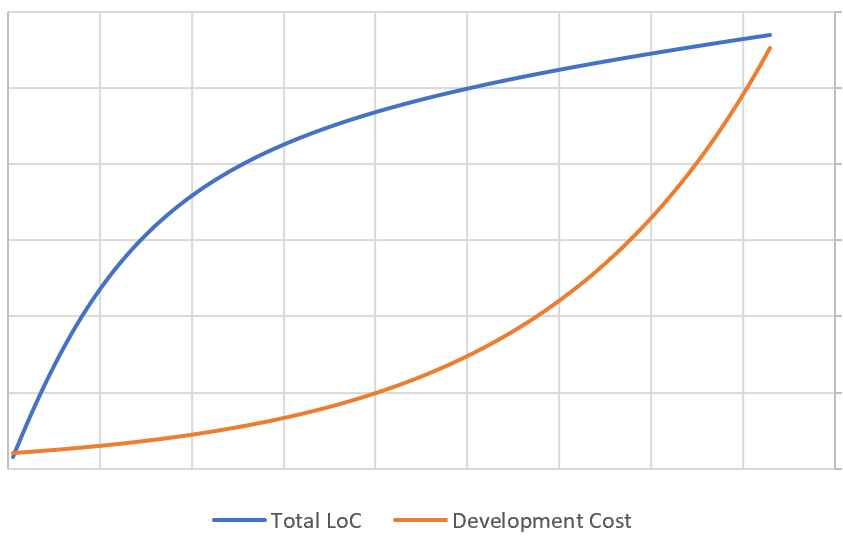
\includegraphics[height=0.75\paperheight]{viscous_growth}
\end{frame}
}

% Notes:

% Viscous growth demonstrates itself in a reduced rate of new features.  Often,
% management may try to fix this issue by adding more engineers to the project,
% but this usually results in increasing development cost while barely
% offsetting the reduction in feature releases.

% Worse, fixing this issue loos to management (and customers) like a failure to
% release new features; product stagnation.  So, developers that try to fix the
% underlying issues are often the first to go, either because of their own
% frustration, or the frustration of management.

%%%%%%%%%%%%%%%%%%%%%%%%%%%%%%%%%%%%%%%%%%%%%%%%%%%%%%%%%%%%%%%%%%%%%%%%%%%%%%%%

{%
\usebackgroundtemplate{%
    \tikz\node[opacity=0.2]{%
        \includegraphics<handout:0>[height=\paperheight,width=\paperwidth]{%
            \background}};}%
\begin{frame}{Viscosity}

    \begin{itemize}
        \item<1->Viscous Design
        \begin{itemize}
            \item<3->When making changes, preserving the design is difficult
            \item<4->When a more correct solution is not the easier solution
            \item<5->\textit{"That is the right way to do this, but we can't do
                that in this project"}
        \end{itemize}
        \item<2->Viscous Environment
        \begin{itemize}
            \item<6->Long builds can prevent people from making the appropriate
                change since it will trigger a longer build.
            \item<7->Slow/unreliable Tests \textit{"I can't run these tests
                after each change, I'd get no work done.  Besides, they always
                fail anyway."}
            \item<8->Slow/cumbersome tools (e.g. large complicated files may
                require longer static analysis)
        \end{itemize}
    \end{itemize}
\end{frame}
}

%%%%%%%%%%%%%%%%%%%%%%%%%%%%%%%%%%%%%%%%%%%%%%%%%%%%%%%%%%%%%%%%%%%%%%%%%%%%%%%%

{%
\usebackgroundtemplate{%
    \tikz\node[opacity=0.2]{%
        \includegraphics<handout:0>[height=\paperheight,width=\paperwidth]{%
            \background}};}%
\begin{frame}{Viscosity}
    \begin{itemize}
        \item Viscous Policies
        \begin{itemize}
            \item<1->Management steps in to avoid the issues above
            \item<2->\textit{"We cannot afford to have anyone touch the
                Fobnicator stack, because too many things depend upon it"}
            \item<3->Policies can remain long after the original problem was
                solved.
            \item<4->Process can also result in viscosity.
            \begin{itemize}
                \item<5->What code changes require stricter review?
                \item<6->What code changes require new or updated documentation?
                \item<7->When does a code revision require upfront design?
            \end{itemize}
        \end{itemize}
    \end{itemize}
\end{frame}
}

% Notes

% If a more correct solution triggers a heavier round of reviews, the incorrect
% solution that can get by with less review and documentation will be favored by
% the developers.  E.g. Creating a new module requires upfront design review.
% Adding the same code inside an existing module requires only the normal code
% review.

%%%%%%%%%%%%%%%%%%%%%%%%%%%%%%%%%%%%%%%%%%%%%%%%%%%%%%%%%%%%%%%%%%%%%%%%%%%%%%%%

{%
\usebackgroundtemplate{%
    \tikz\node[opacity=0.2]{%
        \includegraphics<handout:0>[height=\paperheight,width=\paperwidth]{%
            \background}};}%
\begin{frame}{Viscosity}
    Software develops along the path of least resistance.  If hacks are easier,
            that's what your project will consist of.
\end{frame}
}

%%%%%%%%%%%%%%%%%%%%%%%%%%%%%%%%%%%%%%%%%%%%%%%%%%%%%%%%%%%%%%%%%%%%%%%%%%%%%%%%

\section[Class Design]{Principles of Object Oriented Class Design}

%%%%%%%%%%%%%%%%%%%%%%%%%%%%%%%%%%%%%%%%%%%%%%%%%%%%%%%%%%%%%%%%%%%%%%%%%%%%%%%%

\begin{frame}{\secname}
    SOLID Principles
    \begin{itemize}
        \pause \item \textbf{S}\textit{ingle Responsibility Principle} (SRP)
        \pause \item \textbf{O}\textit{pen Closed Principle} (OCP)
        \pause \item \textbf{L}\textit{iskov Substitution Principle} (LSP)
        \pause \item \textbf{I}\textit{nterface Segregation Principle} (ISP)
        \pause \item \textbf{D}\textit{ependency Inversion Principle} (DIP)
    \end{itemize}
\end{frame}

%%%%%%%%%%%%%%%%%%%%%%%%%%%%%%%%%%%%%%%%%%%%%%%%%%%%%%%%%%%%%%%%%%%%%%%%%%%%%%%%

\subsection{Single Responsibility Principle}

%%%%%%%%%%%%%%%%%%%%%%%%%%%%%%%%%%%%%%%%%%%%%%%%%%%%%%%%%%%%%%%%%%%%%%%%%%%%%%%%

\begin{frame}{\subsecname}

    Responsibility
    \begin{itemize}
        \pause \item Cohesion
        \pause \item Reason to change
        \pause \item Axis of change
    \end{itemize}

\end{frame}

%%%%%%%%%%%%%%%%%%%%%%%%%%%%%%%%%%%%%%%%%%%%%%%%%%%%%%%%%%%%%%%%%%%%%%%%%%%%%%%%

\begin{frame}{\subsecname}

    \begin{minipage}{\columnwidth}
        \cppFile{srp1.cpp}
    \end{minipage}

\end{frame}

%%%%%%%%%%%%%%%%%%%%%%%%%%%%%%%%%%%%%%%%%%%%%%%%%%%%%%%%%%%%%%%%%%%%%%%%%%%%%%%%

\begin{frame}{\subsecname}

    \begin{minipage}{\columnwidth}
        \cppFile{srp2.cpp}
    \end{minipage}

\end{frame}

%%%%%%%%%%%%%%%%%%%%%%%%%%%%%%%%%%%%%%%%%%%%%%%%%%%%%%%%%%%%%%%%%%%%%%%%%%%%%%%%

\begin{frame}{\subsecname}

    \begin{minipage}{\columnwidth}
        \cppFile{srp3.cpp}
    \end{minipage}

\end{frame}

%%%%%%%%%%%%%%%%%%%%%%%%%%%%%%%%%%%%%%%%%%%%%%%%%%%%%%%%%%%%%%%%%%%%%%%%%%%%%%%%

\begin{frame}{\subsecname}

    \begin{minipage}{\columnwidth}
        \cppFile{srp4.cpp}
    \end{minipage}

\end{frame}

%%%%%%%%%%%%%%%%%%%%%%%%%%%%%%%%%%%%%%%%%%%%%%%%%%%%%%%%%%%%%%%%%%%%%%%%%%%%%%%%

\begin{frame}{\subsecname}
    Caution:
    \begin{itemize}
        \pause \item Too much splitting of modules can lead to an overly
            complicated design.
        \pause \item If the code does not change in a way that the two
            responsibilities change at different times, then there's no need to
            separate.
    \end{itemize}
\end{frame}

%%%%%%%%%%%%%%%%%%%%%%%%%%%%%%%%%%%%%%%%%%%%%%%%%%%%%%%%%%%%%%%%%%%%%%%%%%%%%%%%

\subsection{Open Closed Principle}

%%%%%%%%%%%%%%%%%%%%%%%%%%%%%%%%%%%%%%%%%%%%%%%%%%%%%%%%%%%%%%%%%%%%%%%%%%%%%%%%

\begin{frame}{\subsecname}

    \begin{itemize}
        \pause \item "Open for Extension"
        \begin{itemize}
            \pause \item Behavior of the module can be modified through
                extension
        \end{itemize}
        \pause \item "Closed for Modification"
        \begin{itemize}
            \pause \item Extending the behavior requires no change in source
                code or binary executables.
        \end{itemize}
    \end{itemize}

\end{frame}

%%%%%%%%%%%%%%%%%%%%%%%%%%%%%%%%%%%%%%%%%%%%%%%%%%%%%%%%%%%%%%%%%%%%%%%%%%%%%%%%

\begin{frame}{\subsecname}
    \centering
    \includegraphics[height=0.1\textheight]{ocp}
    \begin{itemize}
        \pause \item Client depends on server
        \pause \item Changing server requires modification of client
        \pause \item Use of clients with different servers requires duplication
            of code
    \end{itemize}
\end{frame}

%%%%%%%%%%%%%%%%%%%%%%%%%%%%%%%%%%%%%%%%%%%%%%%%%%%%%%%%%%%%%%%%%%%%%%%%%%%%%%%%

\begin{frame}{\subsecname}
    \centering
    \includegraphics[height=0.2\textheight]{ocp1}
    \begin{itemize}
        \pause \item Enables client implementations for multiple servers
    \end{itemize}
\end{frame}

%%%%%%%%%%%%%%%%%%%%%%%%%%%%%%%%%%%%%%%%%%%%%%%%%%%%%%%%%%%%%%%%%%%%%%%%%%%%%%%%

\begin{frame}{\subsecname}
    \begin{minipage}{\columnwidth}
        \cFile{shape.c}
    \end{minipage}
\end{frame}

%%%%%%%%%%%%%%%%%%%%%%%%%%%%%%%%%%%%%%%%%%%%%%%%%%%%%%%%%%%%%%%%%%%%%%%%%%%%%%%%

\begin{frame}{\subsecname}
    \begin{minipage}{\columnwidth}
        \cFile{shape_comment.c}
    \end{minipage}
\end{frame}

%%%%%%%%%%%%%%%%%%%%%%%%%%%%%%%%%%%%%%%%%%%%%%%%%%%%%%%%%%%%%%%%%%%%%%%%%%%%%%%%

\begin{frame}{\subsecname}

    \begin{minipage}{\columnwidth}
        \cFile{draw_shapes.c}
    \end{minipage}

\end{frame}

%%%%%%%%%%%%%%%%%%%%%%%%%%%%%%%%%%%%%%%%%%%%%%%%%%%%%%%%%%%%%%%%%%%%%%%%%%%%%%%%

\begin{frame}{\subsecname}

    \begin{minipage}{\columnwidth}
        \cFile{draw_shapes_comment.c}
    \end{minipage}

\end{frame}

%%%%%%%%%%%%%%%%%%%%%%%%%%%%%%%%%%%%%%%%%%%%%%%%%%%%%%%%%%%%%%%%%%%%%%%%%%%%%%%%

\begin{frame}{\subsecname}

    \begin{minipage}{\columnwidth}
        \cFile{shape_fix.c}
    \end{minipage}

\end{frame}

%%%%%%%%%%%%%%%%%%%%%%%%%%%%%%%%%%%%%%%%%%%%%%%%%%%%%%%%%%%%%%%%%%%%%%%%%%%%%%%%

\begin{frame}{\subsecname}

    \begin{minipage}{\columnwidth}
        \cFile{draw_shapes_fix.c}
    \end{minipage}

\end{frame}

%%%%%%%%%%%%%%%%%%%%%%%%%%%%%%%%%%%%%%%%%%%%%%%%%%%%%%%%%%%%%%%%%%%%%%%%%%%%%%%%

\subsection{Liskov Substitution Principle}

%%%%%%%%%%%%%%%%%%%%%%%%%%%%%%%%%%%%%%%%%%%%%%%%%%%%%%%%%%%%%%%%%%%%%%%%%%%%%%%%

\begin{frame}{\subsecname}
Subtypes are substitutable for their base types. \pause

If A is a base class, and B inherits from A, then B can be used as A.\pause

Don't surprise users with unexpected changes in behavior.
\end{frame}

%%%%%%%%%%%%%%%%%%%%%%%%%%%%%%%%%%%%%%%%%%%%%%%%%%%%%%%%%%%%%%%%%%%%%%%%%%%%%%%%

\begin{frame}{\subsecname}

    \begin{minipage}{\columnwidth}
        \cFile{lsp_1.c}
    \end{minipage}

\end{frame}

%%%%%%%%%%%%%%%%%%%%%%%%%%%%%%%%%%%%%%%%%%%%%%%%%%%%%%%%%%%%%%%%%%%%%%%%%%%%%%%%

\begin{frame}{\subsecname}

    \begin{minipage}{\columnwidth}
        \cFile{lsp_2.c}
    \end{minipage}

\end{frame}

%%%%%%%%%%%%%%%%%%%%%%%%%%%%%%%%%%%%%%%%%%%%%%%%%%%%%%%%%%%%%%%%%%%%%%%%%%%%%%%%

\begin{frame}{\subsecname}

    \begin{minipage}{\columnwidth}
        \cFile{lsp_3.c}
    \end{minipage}

\end{frame}

%%%%%%%%%%%%%%%%%%%%%%%%%%%%%%%%%%%%%%%%%%%%%%%%%%%%%%%%%%%%%%%%%%%%%%%%%%%%%%%%

\begin{frame}{\subsecname}
    Contract for set\_height():
    \begin{itemize}
        \pause \item Pre-conditions:
        \begin{itemize}
            \pause \item Valid object pointer
            \pause \item 0 <= new height value
        \end{itemize}
        \pause \item Post-conditions:
        \begin{itemize}
            \pause \item Height matches the new value
            \pause \item Width is unchanged
        \end{itemize}
    \end{itemize}
\end{frame}

%%%%%%%%%%%%%%%%%%%%%%%%%%%%%%%%%%%%%%%%%%%%%%%%%%%%%%%%%%%%%%%%%%%%%%%%%%%%%%%%

\subsection{Interface Segregation Principle}

%%%%%%%%%%%%%%%%%%%%%%%%%%%%%%%%%%%%%%%%%%%%%%%%%%%%%%%%%%%%%%%%%%%%%%%%%%%%%%%%

\begin{frame}{\subsecname}
    Allow users to use the parts of your library they need without concern over
    the parts they don't need.
\end{frame}

%%%%%%%%%%%%%%%%%%%%%%%%%%%%%%%%%%%%%%%%%%%%%%%%%%%%%%%%%%%%%%%%%%%%%%%%%%%%%%%%

\subsection{Dependency Inversion Principle}

%%%%%%%%%%%%%%%%%%%%%%%%%%%%%%%%%%%%%%%%%%%%%%%%%%%%%%%%%%%%%%%%%%%%%%%%%%%%%%%%

\begin{frame}{\subsecname}
    Depend upon abstractions.  \pause Do not depend upon concretions.
\end{frame}

%%%%%%%%%%%%%%%%%%%%%%%%%%%%%%%%%%%%%%%%%%%%%%%%%%%%%%%%%%%%%%%%%%%%%%%%%%%%%%%%

\begin{frame}{\subsecname}
    \centering
    \includegraphics[height=0.3\textheight]{ocp_dip}
\end{frame}

%%%%%%%%%%%%%%%%%%%%%%%%%%%%%%%%%%%%%%%%%%%%%%%%%%%%%%%%%%%%%%%%%%%%%%%%%%%%%%%%

\begin{frame}{\subsecname}
    \centering
    \includegraphics[height=0.8\textheight]{dip1}
\end{frame}

%%%%%%%%%%%%%%%%%%%%%%%%%%%%%%%%%%%%%%%%%%%%%%%%%%%%%%%%%%%%%%%%%%%%%%%%%%%%%%%%

\begin{frame}{\subsecname}
    \centering
    \includegraphics[height=0.8\textheight]{dip2}
\end{frame}

%%%%%%%%%%%%%%%%%%%%%%%%%%%%%%%%%%%%%%%%%%%%%%%%%%%%%%%%%%%%%%%%%%%%%%%%%%%%%%%%

\section{Package Design}

%%%%%%%%%%%%%%%%%%%%%%%%%%%%%%%%%%%%%%%%%%%%%%%%%%%%%%%%%%%%%%%%%%%%%%%%%%%%%%%%

\begin{frame}{Principles of Package Architecture}
    Package Principles
    \begin{itemize}
        \item<2-> Package Cohesion
            \begin{itemize}
                \item<4-> Release Reuse Equivalency Principle (REP)
                \item<5-> Common Closure Principle (CCP)
                \item<6-> Common Reuse Principle (CRP)
            \end{itemize}
        \item<3-> Package Coupling
            \begin{itemize}
                \item<7-> Acyclic Dependencies Principle (ADP)
                \item<8-> Stable Dependencies Principle (SDP)
                \item<9-> Stable Abstractions Principle (SAP)
            \end{itemize}
    \end{itemize}
\end{frame}

%%%%%%%%%%%%%%%%%%%%%%%%%%%%%%%%%%%%%%%%%%%%%%%%%%%%%%%%%%%%%%%%%%%%%%%%%%%%%%%%

\begin{frame}{\subsecname}
\end{frame}

%%%%%%%%%%%%%%%%%%%%%%%%%%%%%%%%%%%%%%%%%%%%%%%%%%%%%%%%%%%%%%%%%%%%%%%%%%%%%%%%

\section{Architecture Design}

%%%%%%%%%%%%%%%%%%%%%%%%%%%%%%%%%%%%%%%%%%%%%%%%%%%%%%%%%%%%%%%%%%%%%%%%%%%%%%%%

\begin{frame}{Principles of Package Architecture}
\end{frame}

%%%%%%%%%%%%%%%%%%%%%%%%%%%%%%%%%%%%%%%%%%%%%%%%%%%%%%%%%%%%%%%%%%%%%%%%%%%%%%%%

\section{Conclusion}

%%%%%%%%%%%%%%%%%%%%%%%%%%%%%%%%%%%%%%%%%%%%%%%%%%%%%%%%%%%%%%%%%%%%%%%%%%%%%%%%

\begin{frame}{Principles of Package Architecture}
\end{frame}

%%%%%%%%%%%%%%%%%%%%%%%%%%%%%%%%%%%%%%%%%%%%%%%%%%%%%%%%%%%%%%%%%%%%%%%%%%%%%%%%

\begin{frame}{References}
    \begin{itemize}
        \item \url{https://fi.ort.edu.uy/innovaportal/file/2032/1/design_principles.pdf}
        \item \url{http://www.butunclebob.com/ArticleS.UncleBob.PrinciplesOfOod}
        \item \url{http://notherdev.blogspot.com/2013/07/code-smells-rigidity.html}
        \item \url{https://dev.to/bob/how-do-you-know-your-code-is-bad}
        \item \url{http://staff.cs.utu.fi/~jounsmed/doos_06/slides/slides_060321.pdf}
        \item \url{https://softwareengineering.stackexchange.com/questions/357127/clear-examples-for-code-smells}
    \end{itemize}
\end{frame}

%%%%%%%%%%%%%%%%%%%%%%%%%%%%%%%%%%%%%%%%%%%%%%%%%%%%%%%%%%%%%%%%%%%%%%%%%%%%%%%%

\begin{frame}{Questions}
\end{frame}

\fi
\end{document}

